%%%%%%%%%%%%%%%%%%%%%%%%%%%%%% -*- Mode: Latex -*- %%%%%%%%%%%%%%%%%%%%%%%%%%%%
%% nsf.tex         : 2009 Smart Consumer Proposal
%% Author          : Philip Johnson
%% Created On      : Tue Mar 31 11:16:58 2009
%% Last Modified By: Philip Johnson
%% Last Modified On: Mon Feb 15 17:40:05 2010
%%%%%%%%%%%%%%%%%%%%%%%%%%%%%%%%%%%%%%%%%%%%%%%%%%%%%%%%%%%%%%%%%%%%%%%%%%%%%%%
%%   Copyright (C) 2009 
%%%%%%%%%%%%%%%%%%%%%%%%%%%%%%%%%%%%%%%%%%%%%%%%%%%%%%%%%%%%%%%%%%%%%%%%%%%%%%%
%% 
 
\documentclass[11pt]{article}
\usepackage[final]{graphicx}

\usepackage[nottoc,numbib]{tocbibind}

%% Make subsubsections numbered and included in ToC
\setcounter{secnumdepth}{3}
\setcounter{tocdepth}{3}

\usepackage{multirow}

%% URLs
\usepackage{url}
\usepackage[colorlinks, bookmarks=true]{hyperref}

%% Define a new 'smallurl' style for the package that will use a smaller font.
\makeatletter
\def\url@smallurlstyle{%
  \@ifundefined{selectfont}{\def\UrlFont{\sf}}{\def\UrlFont{\small\ttfamily}}}
\makeatother
%% Now actually use the newly defined style.
\urlstyle{smallurl}

%% CO2 
\usepackage{xspace}
\newcommand{\COtwo}{CO\ensuremath{_2}\xspace}

%% Make margins less ridiculous
\usepackage{fullpage}

%% Since I'm using the LaTeX Makefile that uses dvips, I need this
%% package to make URLs break nicely
\usepackage{breakurl}

\begin{document}
\title{The Kukui Cup: \\Proposal for a UH Dorm Energy Competition}

\author{Philip M. Johnson \\
Collaborative Software Development Laboratory \\
Department of Information and Computer Sciences \\
University of Hawai'i \\
johnson@hawaii.edu \\
\url{http://csdl.ics.hawaii.edu/techreports/10-03/10-03.pdf}
}

\maketitle

\tableofcontents
\newpage

\section{Goals}

We are designing the UH Dorm Energy Competition Project (Kukui
Cup\footnote{We named the competition Kukui Cup because kukui nut oil was used by ancient Hawaiians as a source of light,
  thus serving as the earliest form of ``electricity'' in the islands.}) to achieve three goals:
\begin{enumerate}
\item Improve the {\em energy literacy} of the participating students;
\item Conduct {\em innovative, cutting edge research} in information technology for
  energy-related behavioral change;
\item {\em Save money} for the university by reducing energy costs.
\end{enumerate}

\subsection{Improve energy literacy}

Energy literacy \cite{DeWaters09b, DeWaters09} has three components:
knowledge, attitudes, and behaviors. Energy knowledge refers to factual 
information and skills, such as the ability to estimate the energy savings
in Watt-hours from switching lights from incandescent to compact
flourescent.   Energy attitudes refers to one's opinions and beliefs
related to energy, such as that conserving energy is good for
the environment.   Energy behaviors combine knowledge and attitudes to
produce concrete action, such as replacing the incandescent bulbs in one's
home with compact flourescent. 

While one might assume from the above definition that energy literate
behaviors follow naturally from knowledge and attitudes, there is
substantial research to the contrary.  For example, Geller \cite{Geller81}
performed an experiment in which 40 consumers attended a three hour
workshop on energy conservation.  A pre and post workshop questionnaire
determined that all participants gained greater awareness of energy issues,
more appreciation for what could be done in their homes to reduce energy
use and save money, and a willingness to implement the changes that were
advocated in the workshop. However, a one month followup indicated very
little actual change in behavior. One person lowered the temperature on the
hot water heater. Two additional people had installed insulating blankets
around their hot water heaters, but they had already done this before the
workshop. Finally, eight people installed low-flow shower heads---after all
40 participants had been given the low-flow shower heads at the workshop.

As this and similar research illustrates, simply providing people with
information about energy, even if it affects their attitudes, is generally
not enough to create sustained, positive behavioral change with respect to
their energy usage.  Fortunately, there is also a growing body of research
on techniques that do support behavioral change
\cite{Becker78,Darby06,Faruqui09,Houwelingen89,Peterson07,Peterson07a,Staats04,Vollink99},
which can be summarized as follows.  First, provide {\em personalized
  information} that reflects the consumer's unique circumstances.  For
example, a dorm resident will not respond well to energy tips involving
improved insulation.  Second, provide both {\em general and specific
  commitments}, especially when they can be tied to a broader issue. For
example, pledging to use a clothesline rather than a dryer because it
reduces green house gas emissions.  Third, provide {\em achievable goals}
that can be objectively measured.  An example might be to reduce energy
consumption by 10\% over the previous month.  Fourth, elicit {\em social
  reinforcement} which can be manifested in both overt and subtle ways.
For example, in dorm settings, as more and more residents publicly
participate, it implicitly becomes ``the thing to do''.  Fifth, provide
{\em constant and contextual feedback} which helps verify progress toward
goals and can reinvigorate commitments, as long as the feedback is provided
in the right way at the right time.  Sixth, {\em financial incentives} can
be a powerful motivator for energy conservation. For example, a prize such
as iPods to the members of the dorm floor who conserved the most energy.

Thus, the first design goal of the dorm energy competition is to increase
factual knowledge about energy by participants, foster more sophisticated
attitudes based upon this knowledge, and, most finally, facilitate actual
behavioral change.


\subsection{Conduct innovative IT energy research}

As noted in the previous section, there is evidence in support of a variety
of techniques for promoting sustained, positive behavioral change, but
current dorm energy competitions either do not employ these techniques, or
they do not utilize information technology effectively to deploy the
techniques or support assessment of their effectiveness.

The most common form of information technology support for dorm energy
competitions is a simple relatively static web site, as illustrated in
Figure \ref{fig:wellesley}.  These websites provide access to resources
about energy, and feedback regarding energy usage for the entire building
every few days.  The most sophisticated technology to date is the Campus
Resource Monitoring System at Oberlin College, which has the potential to
provide near-real time energy consumption data\footnote{With respect to
  energy consumption data, we define ``near-real time'' as sub-minute
  update intervals.  For example, obtaining meter data every 10 seconds is
  ``near real time'', while obtaining meter data every 15 minutes is not.}.

\begin{figure*}[!ht]
  \center
  \includegraphics[width=0.8\textwidth]{wellesley.ppt.eps}
  \caption{\em \small The Wellesley College Dorm Energy Competition Web site.}
 \label{fig:wellesley}
\end{figure*} 


We are designing a collection of software services that will provide UH
dorm residents participating in the competition with unparalleled
information technology support for improving their energy literacy.  Our
software will support a unique combination of features including: (a)
near-real time energy consumption data, (b) floor-level as well as
building-level energy data; (c) personalized, login-protected pages for
each student; (d) energy literacy activities with a ``Kukui Nut'' award
system for participation; and (e) integration with other information
technologies used by students, including text messaging, Facebook, email,
and Twitter.

Our software services are not designed merely to be cool or trendy; they
are designed to enable substantial, important research into energy
behavior. While prior research has generated evidence regarding a variety
of techniques for fostering behavioral change, there is relatively little
understanding of the relative importance or impact of these methods.  Our
software will enable us to present students with a variety of avenues for
participation and incentives and then track many of the ways in which they
participated. It will enable us to observe and record participant energy
usage (on a floor-by-floor basis) before, during, and after the
competition.  In addition, we will request student volunteers for an energy
literacy assessment both before and after the competition.  The result of
these three streams of data will provide a uniquely rich source of insight
into the popularity of various activities, their impact on energy literacy,
and the final impact on actual energy usage.

More details on the software are provided below, but in summary, the goal
of our software is to provide innovative support for improving energy
literacy in students combined with infrastructure to enable ground-breaking
empirical research in sustainability and energy.

\subsection{Save money}

The final goal is to save money.  Previous dorm energy challenges at
Brandeis University, Carleton College, Harvard University, MIT, Mount
Holyoke College, Ohio University, and Williams College have reported energy
savings, generally in the range of 7\% to 16\%.  If we can achieve these
results, and if the savings can be sustained for the remainder of the
school year, then energy costs for the dorms alone could be reduced by tens
of thousands of dollars.

However, those are just the ``first-order'' savings to the university.  If
the competition achieves the goal of improving the energy literacy of
students, then their energy literate behavior will be manifested everywhere
on campus, not just in their dorm floors.  A more energy literate student
will choose energy saving behaviors in campus cafeterias, classrooms, and
labs, producing additional, ``second-order'' savings to the university.
Furthermore, the ``return on investment'' in improved energy literacy will
occur over their entire time at the university, not just during the one
month competition, and not just during their one year in the dorm.  We also
hope that these energy literate students will influence their friends in
positive ways, reaping additional dividends.

There is even the possibility of ``third-order'' savings.  We are designing
this project to begin with dormitory energy competitions, then extend into
residential community energy challenges \cite{csdl2-09-15}.  In addition,
we are releasing all software developed under this project as open source
in order to facilitate more wide-spread adoption.  Thus, this project could
lead to eventual energy cost savings in our community and elsewhere.

\section{Approach}
\label{sec:approach}

Our pursuit of the three goals of energy literacy, innovative research, and
saving money results in the following proposed approach to a UH Dorm
Energy competition.  

To summarize, we propose to hold the first annual UH Dorm Competition
during Fall semester of 2010.  The first competition will involve just two
of the freshman dormitories. We will conduct focus groups in these dorms this
spring to gain buy-in and feedback from current residents and Resident
Advisors.  During the summer, floor-level energy metering will be installed
in the selected dorms.  During early fall, a specialized web application
will become available. The competition will be held during the month of
October, 2010.  We will continue to monitor energy usage for the remainder
of the year and conduct follow-up studies to assess the impact and
permanence of any energy reductions observed during the competition period.

We plan to build upon the results from the first year to hold improved
versions in following years, hopefully expanding the number of involved
dorms as well. 

\subsection{User Interface}
\label{sec:userinterface}

We plan to embed the Dorm Energy Competition within a more general web
application called ``University of Hawaii Dorm Energy''.  This site will,
in addition to competition data, provide general information and resources
about dorm energy usage on a year-around basis.   Figure \ref{fig:homepage}
illustrates a mockup of the home page for this site. 

\begin{figure*}[!ht]
  \center
  \includegraphics[width=1.0\textwidth]{home.tiff.eps}
  \caption{\em \small A mockup of the home page.}
 \label{fig:homepage}
\end{figure*} 

This public home page provides general information about energy usage, and
tabs to other pages including: a Resource page with links to further
information about energy usage and conservation; an Energy Data page that
displays charts generated from meter data; a Kukui Cup page that will
present current standings and activities related to the competition during
October, and more general information about it at other times of the year;
and a Help page that provides contact information.

{\em More screen shots will be described here once they are available.}

For more details on the site and its functionality, see Section \ref{sec:features}.

\subsection{Architecture}

The primary hardware and software components are summarized in Figure \ref{fig:architecture}.

\begin{figure*}[!ht]
  \center
  \includegraphics[width=1.0\textwidth]{architecture.ppt.eps}
  \caption{\em \small Basic architecture of the dorm energy data collection system.}
 \label{fig:architecture}
\end{figure*} 

An energy meter will be installed on each floor of each dorm involved in
the competition.  Section \ref{sec:meters} presents the results of our
research so far on appropriate commercial meters for this installation. 

Each meter will have an ethernet connection, and energy data from each
meter will be sent at sub-minute intervals to our software service,
WattDepot \cite{WattDepot}.  We directly connect each meter via Ethernet,
rather than use a building-wide ModBus with a single Ethernet gateway, in
order to avoid bus contention that might occur due to the sub-minute
polling requirements for our system.

The energy data collected from each floor of each dorm at sub-minute
intervals is stored in WattDepot, which can perform various analyses
including aggregation and interpolation to transform it into a
convenient form for display within the web application.

We recognize that several aspects of our proposed architecture are unusual:
installing meters on every floor (versus one for the entire building);
directly connecting each meter to Ethernet (versus using ModBus or a mesh
network); and sub-minute polling (versus 15 minute or greater polling).
These decisions are based upon our research into effective incentives for
sustained, positive behavioral change, which includes personalized,
constant, and contextual feedback.  

As a simple example, let's say that the residents of a dorm floor want to
figure out their ``baseline'' energy usage: how much electricity is used on
their floor after they turn off everything under their control.  If the
only meter available is at the building-level, the residents could not
succeed, since energy fluctuations in the remainder of the building would
drown out their action.  Similarly, if energy data from the meters is collected
only once every 15 minutes, the experiment becomes difficult to perform,
since they would have to keep everything off for an extended period of
time.  

Other behavioral incentives affected by this architecture include
personalized information and social norms.  By providing floor-level
meters, we can support competition between floors as well as between dorms.
This finer granularity of competition makes the actions of any individual
vastly more significant, since they are one of 12 members, as opposed to
one of 200 or more.

\subsection{Meters}
\label{sec:meters}

This proposal requires the installation of energy meters on each floor of
the dorms participating in the competition.  We conducted a review of
commercial building meters to determine which ones might be
suitable.  To support this process, we developed the list of
requirements summarized in Figure \ref{fig:meterrequirements} below:

\begin{figure}[!ht]
\small
\begin{tabular}{p{1.75in}p{4.25in}} \hline
{\bf Requirement} & {\bf Description}  \\
Total meters & 24 (estimate based on 2 dorms with 12 floors each) \\ 
Building power (BP) & 3 phase \\  
Max current (MC) & 500 amps (estimated)  \\ 
Required data (RD) & kW (instantaneous power); kWh (cumulative energy usage) \\ 
Data sampling interval (DSI) & Every 10 seconds (desired); sub-minute (required) \\ 
Network comm. (NC) & TCP/IP via Ethernet (desired); WiFi (possibly acceptable) \\ 
Internal storage (IS) & Optional, but desirable in case internet connection
goes down. Historical data not needed at sub-minute intervals. \\ 
Submetering (SM) & Optional, but desirable in case we want to track a shared
resource (laundry room) separately \\ 
Software Interface (SI) & Two options: (1) The meter can be configured to emit
an HTTP POST at specified sampling interval; or (2) the vendor provides an
API that we can use to query the device at the data sampling interval. \\ \hline
\end{tabular} 
\normalsize
\caption{{\em Meter requirements}}
\label{fig:meterrequirements}
\end{figure}

Based upon these requirements, we contacted a variety of vendors to see
which of their models could satisfy these requirements.  Figure
\ref{fig:meterresults} summarizes our current findings.  

\begin{figure}[!ht]
\small
\begin{tabular}{l l l l l l l l l l } \hline
{\bf Company/Meter }          & {\bf BP } & {\bf MC} & {\bf RD} & {\bf DSI} & {\bf NC} & {\bf IS} & {\bf SM} & {\bf SI} & {\bf Cost/meter}   \\ 
Accu-Energy/Acuvim IIR       &   X           &           X    &           X   &          X    &          X     &         X   &          X    &         X   &        \$1359 \\ 
Electro Ind./Shark 200S        &      X        &           X    &           X   &          X    &          X     &         X   &          X    &         X   &        \$1295 \\ \hline \hline
Yokogawa/PR300                  &      X        &           X    &           X   &          X    &          X     &              &          X    &         ?   &          ? \\  
Quad-Logic/MiniCloset 5C   &   X           &           X    &           X   &          X    &          X     &        X    &          X    &         X   &         \$3100 \\  
PowerLogic/PM800                &      X        &           X    &           X   &          X    &          X     &       X     &          X    &             &          \$3889 \\  
Dent/PowerScout                   &      X        &           X    &           X   &          X    &          X     &              &          X    &             &          \$535 \\  
Microdaq/Elite Pro                 &      X        &           X    &           X   &          X    &          X     &      X     &              &               &          \$995 \\  
D-Mon/Class 2000                 &      X       &           X    &           X   &                &                 &         X    &          X    &              &          \$940 \\  \hline
\end{tabular} 
\normalsize
\caption{{\em Meter Results. Those above the double line appear best suited for this application. }}
\label{fig:meterresults}
\end{figure}

We have prepared a separate technical report \cite{Lim10} that provides details on our meter research and how we came to these conclusions. 

\subsection{Web application features}
\label{sec:features}

Section \ref{sec:userinterface} provides a sense for the look-and-feel of
the web application through a small selection of screen shots.  This section
summarizes the functionality of the system.

\paragraph{General UH dorm energy information (year round).}  The system will provide a set of public pages that provide residents and community members with general information about dorm energy usage, including: (a) charts with current and historical energy usage data; (b) pointers to online references relevant to dorm energy issues; and (c) who to contact for more information.  For the two dorms in which energy meters will be installed, we will collect energy usage data automatically.  For other dorms, we hope that building-level energy meters are available that we can read manually on a weekly basis and input into WattDepot, so that aggregate energy usage data for all UH dorms can be made available from this website.

\paragraph{Kukui Cup competition (October only).}  During October of each
year, the system will provide specialized features to support the Kukui Cup
competition.  These features include: (a) login-protected, personal pages
for residents in participating dorms; (b) login-protected, admin pages for
monitoring the competition and/or updating pages; (c) current standings for
an ``Energy Conservation'' competition, in which individual floors compete
against each other to reduce their energy usage; and (d) current standings
for a ``K-Nuts'' competition, in which individual floors compete against
each other to obtain the highest number of Kukui Nuts through engaging in
energy literacy-related activities.  The next paragraphs look at these
components of the Kukui Cup competition in a bit more detail.
 
\paragraph{Login-protected, personal pages.}  In September, the system will
be configured with a list of UH accounts corresponding to the residents of
the dorms participating in the Kukui Cup.  When a dorm resident logs in to
the Dorm Energy web site (using the UH Web Login service), they are taken
to a personalized page that provides meter data for their floor, their
floor's current standings in both the Energy Conservation and K-Nuts
competitions, and activities they can carry out to improve their standings.

\paragraph{Login-protected, admin pages.}  The system is also configured
with a set of UH accounts whose owners are provided with administrator
privileges on the site.  This enables them to edit public pages and award
K-Nuts to students who have successfully completed activities.

\paragraph{The Energy Conservation competition.}  One of two competitions
held during October, the Energy Conservation competition awards a variety
of prizes to the floor that reduces their energy consumption the most.

\paragraph{The K-Nut competition.}  While the energy conservation
competition rewards participants only on the basis of reduced energy usage,
the K-Nut competition rewards participants for energy literacy activities. 

\subsection{Development Timeline}

Figure \ref{fig:timeline} presents the major activities and milestones  for the next twelve months of this project.

\begin{figure}[!ht]
\small
\begin{tabular}{p{1in}p{5in}} \hline
{\bf Month} & {\bf Activities}  \\
March, 2010 &  Refine proposal, decide on dormitories that will
participate in competition, obtain approval from UH Housing and UH Facilities to proceed with competition development. \\

April, 2010 & Conduct focus group meetings with current
dormitory residents and RAs to obtain feedback on site and competition
design. \\

May, 2010 &  In collaboration with UH Facilities, decide upon meter model to install and order. \\

July, 2010 & Install meters in dormitories.  Verify that WattDepot collection and analysis facilities work correctly. \\

August, 2010 & Bring Dorm Energy website online.  Configure website with information about all residents; test logins.  Conduct meetings with RAs and Housing staff to lay groundwork for October competition. \\

September, 2010 & Finish planning competition events.  Carry out pre-contest publicity activities.  Install LCD display in entrance way to dormitory that will provide real-time competition and energy usage information.    \\

October, 2010 & Competition takes place! \\

November, 2010 &  Immediate post-contest feedback and analysis.  \\

February, 2011 &  Delayed post-contest feedback and analysis (to determine longer-term retention of energy literacy.)  \\ \hline
\end{tabular} 
\normalsize
\caption{{\em Project timeline}}
\label{fig:timeline}
\end{figure}

\subsection{Stakeholders}

There are a variety of stakeholders in this project whose needs must be satisfied. 


\subsection{Budget}

Figure \ref{fig:budget} presents the proposed cost items for this project:

\begin{figure}[!ht]
\small
\begin{tabular}{lrl} \hline
{\bf Item }              & {\bf Cost }  & \\ 
Meters (hardware) & \$36,000 & (estimate based upon 24 meters at \$1,500 each) \\
Meters (installation) & \$12,000 & (estimate based upon 1 hour installation per meter at \$50 per hour) \\
Prizes                   & \$2,000 & (estimate based upon 20 prizes at \$100/each) \\ \hline 
{\em Total}          &  {\em \$50,000} & \\ \hline      
\end{tabular} 
\normalsize
\caption{{\em Project budget.}}
\label{fig:budget}
\end{figure}

For the first line item, Meters (hardware), we will pursue funding from the
following sources: an NSF grant submitted by Philip Johnson (currently
under review); REIS (Renewable Energy and Island Sustainability) project;
Blue Planet Foundation; University of Hawaii Office of Sustainability.

For the second line item, Meters (installation), we will request in-kind donation 
of labor and personnel from  University of Hawaii Facilities Management.

For the third line item, Prizes, we will solicit in-kind donation of prizes from
local businesses.




\subsection{Aligning incentives and design components}

To conclude Section \ref{sec:approach}, it might be useful to review how the
elements of this project relate to the research objectives.  Figure
\ref{fig:incentives} summarizes the components of our design and how they
together satisfy each of the six behavioral incentives listed previously:

\begin{figure}[!ht]
\small
\begin{tabular}{p{3in}p{3in}} \hline
{\bf Design Component} & {\bf Behavioral Incentive}  \\
Near-real time energy data & constant feedback \\
Floor-level data & contextual feedback  \\
Personalized (login-protected) home pages  & personalized information \\
Competition commitments & general and specific commitments \\
Competition goals & achievable goals \\
Kukui Nut competition & social reinforcement \\
Energy use competition & social reinforcement \\
Competition prizes & financial incentives  \\ \hline
\end{tabular}
\normalsize
\caption{{\em Design components and how they satisfy various incentives for behavioral change}}
\label{fig:incentives}
\end{figure}

\section{Final thoughts: Why care about behavior?}

There is a school of thought that views human behavior as too difficult to
change and ultimately unreliable, and that the only realistic approach to
energy conservation is through ``top-down'' incorporation of new technology
that eliminates the need for human decision-making/behavior.  For example,
to reduce energy in the dorm, the best approach is to have the Housing
Office and Facilities Management improve the efficiency of air
conditioning, replace the light bulbs, increase the amount of insulation,
and so forth.

We certainly agree that the introduction of new technology is desirable and
should be done whenever possible.  Indeed, a study by Granade \cite{Granade09}
shows that U.S. energy consumption could be reduced by almost 25\% if
cost-effective energy saving technology already available was implemented.

However, we disagree that behavior is too difficult or leads to only
marginal results.  An old, inefficient air conditioner uses far less energy
than a state-of-the-art unit if an energy literate student decides to turn
it off (or not turn it on at all).  The energy associated with landfill
management is reduced when an energy literate student chooses a
non-styrofoam container, or to bring their own bag to the farmers market.

Finally, we disagree that ``top-down'' approaches are the only viable way
to effect conservation-related change, and suggest that the rapidly growing
organic foods industry provides a compelling example.  There was no
top-down mandate for organic foods in this country. Rather, a growing
number of ``food-literate'' consumers began buying these foods despite
their generally higher price.  The result is annual industry growth of over
20\% for the past several years.  We believe that energy literacy can
catalyze a similar appetite for energy conservation.







\bibliography{smartconsumer,csdl-trs}
\bibliographystyle{plain}
\end{document}
